\chapter{Teknik \textit{Divide and Conquer}}\label{ch:modul4}

\section{Pengenalan \textit{Divide and Conquer}}
\textit{Divide and Conquer} merupakan salah satu pendekatan dalam menyelesaikan permasalahan algoritma. \textit{Divide and Conquer} terdiri atas tiga langkah:
\begin{enumerate}
	\item \textbf{\textit{Divide}/Memecah} --- Sebuah permasalahan yang ada dibagi menjadi permasalahan yang lebih kecil (\textit{subproblem}).
	\item \textbf{\textit{Conquer}/Menyelesaikan} --- Menyelesaikan setiap \textit{subproblem} yang ada secara rekursif. Jika \textit{subproblem} tersebut sangat kecil atau tak bisa dipisahkan lagi, maka diselesaikan secara langsung dengan menggunakan algoritma yang sederhana.
	\item \textbf{\textit{Combine}/Menggabungkan} --- Menggabungkan setiap solusi dari \textit{subproblem} yang telah diselesaikan menjadi sebuah solusi yang lengkap dan optimal.
\end{enumerate}

Teknik \textit{Divide and Conquer} digambarkan dalam Figur \ref{fig:DivideandConquerIllustration}, yang menunjukkan pembagian sebuah masalah menjadi dua submasalah yang lebih sederhana.

\newpage{}
\begin{figure}[htbp]
\begin{center}
	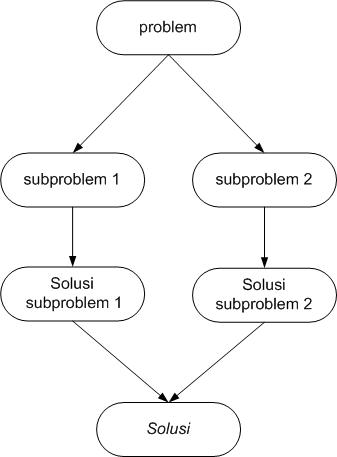
\includegraphics[scale=0.7]{fig/sunario-3/Ilustrasi.jpg}%
	\caption{Illustrasi dari Divide and Conquer}%
	\label{fig:DivideandConquerIllustration}%
\end{center}
\end{figure}

Sebagai Contoh, untuk menghitung total jumlah dari element-element dalam List, kita dapat menggunakan perulangan sederhana:



\lstset{language=Python}
\label{lst:SimpleSum}
\begin{lstlisting}[frame=single]
A = [4,1,3,5,6,7,2]
total = 0
  for i in range(0,len(A)):
    total = total + A[i]
print(total)
\end{lstlisting}

Algoritma perulangan yang digunakan pada kode di atas dapat memberikan hasil yang benar, tetapi terdapat beberapa masalah pada kode tersebut, yaitu perhitungan dilakukan secara linear, yang menghasilkan kompleksitas $O(n)$. Hal ini tentunya cukup ideal untuk ukuran list kecil, tetapi jika ukuran list menjadi besar (beberapa Milyar elemen) maka perhitungan akan menjadi sangat lambat.

Dengan menerapkan Teknik \textit{Divide and Conquer}, maka masalah penjumlahan sebelumnya dapat dibagi menjadi submasalah yang lebih kecil. Langkah pertama yang dapat dilakukan adalah menerapkan teknik rekursif untuk membagi-bagikan masalah menjadi masalah yang lebih kecil. Jika awalnya kita harus menghitung total keseluruhan list satu per satu, sekarang kita dapat melakukan perhitungan dengan memecah-mecah list terlebih dahulu:

\lstset{language=Python}
\label{lst:DivideAndConquerSum}
\begin{lstlisting}[frame=single]
def SumOfList(MyList):
  if len(MyList) <= 1:
    return MyList[0] 
	mid = len(MyList) // 2
  left = SumOfList(MyList[:mid])
  right = SumOfList(MyList[mid:])
  return left + right
	
\end{lstlisting}

Setelah membagikan list menjadi dua bagian terus menerus sampai bagian terkecilnya, penjumlahkan kedua nilai list tersebut dapat dilihat pada Figur \ref{fig:DivideAndConquerSum} berikut:

\begin{figure}[htbp]
\begin{center}
	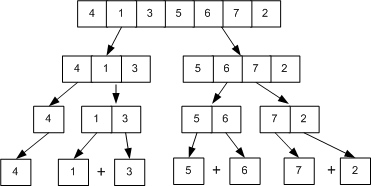
\includegraphics[scale=0.7]{fig/sunario-3/Sum.png}%
	\caption{Illustrasi Penjumlahan Divide and Conquer}%
	\label{fig:DivideAndConquerSum}%
\end{center}
\end{figure}

Algoritma \textit{Divide and Conquer}, jika diimplementasikan menggunakan library atau bahasa yang tepat akan meningkatkan efisiensi algoritma secara logaritmik. Untuk melihat kompleksitas algoritma perhatikan analisis pada fungsi SumOfList dengan teknik \textit{Divide and Conquer} berikut ini:

\lstset{language=Python}
\label{lst:DivideAndConquerSum}
\begin{lstlisting}[frame=single]
def SumOfList(MyList):
  if len(MyList) >= 1:		#cost = a 
    return MyList[0]		#cost = b 
	mid = len(MyList) // 2	#cost = c
  left = SumOfList(MyList[:mid]) #cost = f(n/2) + h
  right = SumOfList(MyList[mid:]) #cost = f(n/2) + i
  return left + right	#cost = d
	
\end{lstlisting}

yang secara matematis dapat dituliskan seperti berikut:
$$	  \mathnormal{f(n) = a+b+c+f(\frac{n}{2})+h+f(\frac{n}{2})+i+d } $$
$$	  \mathnormal{f(n) = 2f(\frac{n}{2})} $$

karena ukuran dari mid adalah panjang list $(n)$ dibagi dua. Dengan begitu, kompleksitas dari algoritma adalah:

\begin{figure}[htbp]
\begin{center}
	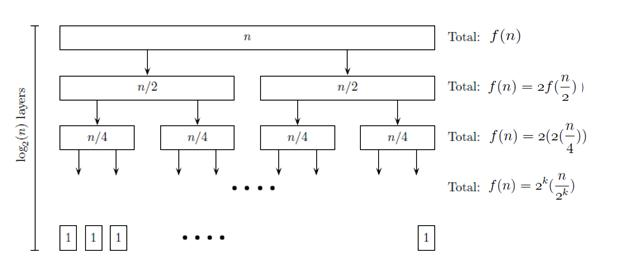
\includegraphics[scale=0.8]{fig/sunario-3/fn.jpg}%
	\caption{Illustrasi pembagian list}%
	\label{fig:PembagianList}%
\end{center}
\end{figure}

dengan syarat berhenti adalah $k \geq 1$ sehingga:

$$	  \mathnormal{ \frac{n}{2^{k}}=1} $$
$$	  \mathnormal{n=2^{k}} $$
$$	  \mathnormal{k=log_{2}n} $$

Dibandingkan dengan Algoritma penjumlahan dengan perulangan $(O(n))$, Kompleksitas dari fungsi penjumlahan dengan teknik \textit{Divide and Conquer} diatas adalah $O(log n)$.

\section{\textit{Binary Search}}
Algoritma \textit{Binary search}  merupakan  algoritma untuk melakukan pencarian pada list yang sudah mempunyai syarat bahwa list sudah terurut, baik secara menaik ataupun menurun. Algoritma \textit{Binary search} menggunakan 3 langkah dari \textit{Divide and Conquer} sebagai berikut:
\begin{enumerate}
\item \textbf{\textit{Divide}} --- Membagi $n$ elemen/bilangan menjadi dua bagian dimana masing-masing adalah $n/2$. Setiap $n$ bilangan akan terus dibagi dua menjadi dua bagian kiri dan kanan hingga data yang dicari ditemukan.
\item \textbf{\textit{Conquer}} --- Cari nilai kunci dalam  List terurut dan mengembalikan indeks di mana kunci itu ditemukan atau -1 jika tidak ditemukan dan membagi List secara rekursif.
\item \textbf{\textit{Combine}} --- Tahap ini tidak perlu dilakukan karena yang diperlukan hanya 1 element berupa data yang dicari.
\end{enumerate}

 Misalnya untuk menemukan nilai dari \textit{Val}  dalam List \textit{MyList} dengan menggunakan Algoritma \textit{Binary search}, maka ada 3 kemungkinan kondisi pada \textit{Binary search} yaitu:
\begin{enumerate}
  \item Jika nilai dari \textit{Val} di temukan pada MyList[middle], maka proses pembagian ruangan berhenti. 
  \item Jika nilai dari \textit{Val} $<$ MyList[middle], maka pencarian di batasi hanya pada bagian sebelah kiri dari List. Seluruh elemen yang berada di sebelah kanan dapat di abaikan.
  \item Jika nilai dari \textit{Val} $>$ MyList[middle], maka pencarian di batasi hanya pada bagian sebelah kanan dari List. Seluruh elemen yang berada di sebelah kiri dapat di abaikan.
  \item Jika seluruh data telah di cari namun nilai dari \textit{Val} tidak ditemukan, maka diberi nilai seperti -1.
\end{enumerate}

Sebagai Contoh, pencarian nilai 15 dari sebuah list dapat dilihat pada Figur \ref{fig:Binary Search Ilustration} berikut:

\begin{figure}[htbp]
\begin{center}
	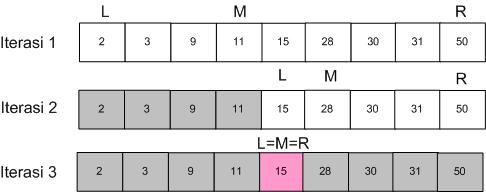
\includegraphics[scale=0.8]{fig/sunario-3/BinarySearch.jpg}%
	\caption{Illustrasi Binary Search}%
	\label{fig:Binary Search Ilustration}%
\end{center}
\end{figure}

\newpage{}
Algoritma \textit{Binary search} dapat diterapkan dengan menggunakan cara rekursif maupun nonrekursif. Untuk cara rekursif dapat diimplementasikan sebagai berikut:

\lstset{language=Python}
\label{lst:BinarySearch}
\begin{lstlisting}[frame=single]
def BinarySearch(MyList, val, left, right):
  if right < left:
    print("%d not found in list"%val)
    return -1
	
  mid = (left + right) // 2
  if MyList[mid] > val:
    return BinarySearch(MyList, val, left, mid-1)
  elif MyList[mid] < val:
    return binary_search(MyList, val, mid+1, right)
  else:
    print("%d found in index %d"%(val, mid))
  
  return mid
\end{lstlisting}

\subsection{Analisis Binary Search}
Untuk analisis metode binary search dalam menentukan kompleksitasnya, perhatikan untuk sebuah list, misalkan dengan panjang $(n) = 8$, maka :\newline
Ketika n=8, Binary Search akan mereduksi ukuran listnya menjadi 4\newline
Ketika n=4, Binary Search akan mereduksi ukuran listnya menjadi 2\newline
Ketika n=2, Binary Search akan mereduksi ukuran listnya menjadi 1\newline

Dapat dilihat bahwa binary search dipanggil sebanyak tiga kali untuk $n = 8$. Sehingga didapat $8 = 2^{3}$ atau secara general dapat dikatakan $n = 2^{k}$.  Nilai dari k dapat dinotasikan menjadi $2^{k} = n$ sehingga $k = log_2\ n$ sehingga didapatkan untuk kompleksitas dari binary search adalah  O (log n).

Misalnya jika kita memiliki list sebanyak $n$ elemen, maka kasus tersebut melakukan pembandingan list sebanyak $log\ n$. Bandingkan dengan linear search yang  melakukan pembandingan sebanyak $n$. Tentunya algoritma binary search menjadi lebih cepat. Namun jika data yang ada merupakan data yang tidak terurut maka akan jauh lebih cepat jika menggunakan linear search sehingga penggunaan binary search akan ada cost tambahan yaitu dalam mengurutkan List.

\section{\textit{Merge Sort}}
Algoritma \textit{Merge Sort} merupakan algoritma pengurutan yang mengikuti pendekatan \textit{Divide and Conquer}. Algoritma tersebut menggunakan 3 langkah dari \textit{Divide and Conquer} sebagai berikut:
\begin{enumerate}
\item \textbf{\textit{Divide}} --- Membagi $n$ elemen/bilangan menjadi dua bagian dimana masing-masing adalah $n/2$. Setiap $n$ bilangan akan terus dibagi dua sampai habis atau bilangan tinggal 1 saja.
\item \textbf{\textit{Conquer}} --- Mengurut setiap bagian secara rekursif menggunakan \textit{merge sort}. 
\item \textbf{\textit{Combine}} --- Menggabungkan dua bagian yang telah diurut untuk menghasilkan satu bagian keseluruhan yang sudah terurut.
\end{enumerate}

Figur \ref{fig:mergeSortIllustration} menggambarkan cara kerja Merge Sort terhadap 4 buah bilangan yang tak terurut. Di illustrasi tersebut \textit{List} yang memiliki 4 bilangan tak terurut dipecah-pecah sampai menjadi 1 buah bilangan atau panjang \textit{List} 1 ($A.length = 1$). Karena satu buah bilangan sudah merupakan bilangan yang terurut maka pecahan bilangan tersebut digabungkan sampai menjadi satu \textit{List} bilangan yang terurut. 

\begin{figure}[htbp]
\begin{center}
	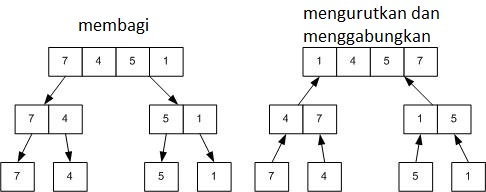
\includegraphics[scale=0.8]{fig/sunario-3/mergeSort1.jpg}%
	\caption{Illustrasi dari cara kerja merge sort}%
	\label{fig:mergeSortIllustration}%
\end{center}
\end{figure}


Algoritma \textit{merge sort} terdiri dari dua algoritma utama yaitu Algoritma (MERGE($left,right$)) dan Algoritma (MERGE-SORT($MyList$)). 

Algoritma MERGE-SORT($MyList$) ditujukan untuk membagi (\textit{divide}) sebuah \textit{List} $MyList$ menjadi dua bagian secara rekursif sampai \textit{List} tersebut tak bisa dibagi lagi (panjang \textit{List} $MyList$ adalah 1). 

\lstset{language=Python}
\label{lst:MargeSort}
\begin{lstlisting}[frame=single]
def merge_sort(A, p, r):
    if p< r:
        q = (p+r)//2
        merge_sort(A, p, q)
        merge_sort(A, q+1, r)
        merge(A,p,q,r)
\end{lstlisting}

Algoritma MERGE($left,right$) ditujukan untuk menggabungkan (\textit{combine}) kumpulan \textit{List} yang sudah diurut (memiliki panjang 1) menjadi sebuah \textit{List} baru yang sudah terurut.

\lstset{language=Python}
\label{lst:Marge}
\begin{lstlisting}[frame=single]
def merge(A,p,q,r):
    n1 = q-p+1
    n2 = r-q
    L =[]
    R =[]
    for i in range(0,n1):
        L.append(A[p+i])
    for j in range(0,n2):
        R.append(A[q+j+1])
    L.append(float("inf"))
    R.append(float("inf"))
    i = 0
    j =0
    for k in range(p, r+1):
        if L[i] <= R[j]:
            A[k] = L[i]
            i = i + 1
        else:
            A[k] = R[j]
            j = j + 1

\end{lstlisting}

Perlu diketahui di algoritma \textit{merge sort} tidak diperlukan fungsi khusus untuk \textit{Conquer} dikarenakan \textit{List} yang memiliki panjang 1 secara otomatis sudah terurut.

\newpage{}
\subsection{Analisis Merge Sort}
Seberapa efisienkah \textit{merge sort}? Berikut analisis dari kompleksitas \textit{merge sort}.

\lstset{language=Python}
\label{lst:MargeSort}
\begin{lstlisting}[frame=single]
def merge_sort(A, p, r):
    if p< r:                    #cost = a
        q = (p+r)//2            #cost = b
        merge_sort(A, p, q)     #cost = f(n/2) + h
        merge_sort(A, q+1, r)   #cost = f(n/2) + i
        merge(A,p,q,r)          #cost = g.n + j
\end{lstlisting}

yang secara matematis dapat dituliskan seperti berikut:
$$	  \mathnormal{f(n) = a+b+f(\frac{n}{2})+h+f(\frac{n}{2})+i+g.n+j } $$
$$	  \mathnormal{f(n) = 2f(\frac{n}{2})+a.n + b} $$

dengan syarat $n > 1$, maka:
$$	  \mathnormal{f(n) = 2f(\frac{n}{2})+a.n } $$
$$	  \mathnormal{f(n) = 2(2f(\frac{n}{4})+a.\frac{n}{2} )} + a.n $$
$$	  \mathnormal{f(n) = 4f(\frac{n}{4})+2a.n } $$
$$	  \mathnormal{f(n) = 4(2f(\frac{n}{8})+a.\frac{n}{4} )}+2a.n $$
$$	  \mathnormal{f(n) = 8f(\frac{n}{8})+3a.n } $$
$$	  \mathnormal{f(n) = 16f(\frac{n}{16})+4a.n } $$
$$	  \mathnormal{f(n) = 2^{k}f(\frac{n}{2^{k}})+k.a.n } $$

untuk $ \mathnormal{f(n) = (\frac{n}{2^{k}})} $ :

$$ \mathnormal{\frac{n}{2^{k}}} $$
$$ \mathnormal{2^{k}=n} $$
$$ \mathnormal{k=log_{2}n} $$

sehingga :

$$	  \mathnormal{f(n) = 2^{log_{2}n}f(1)+log_{2}n.a.n } $$

$$	  \mathnormal{f(n) = a.n\ log\ n = O(n\ log\ n)} $$
 
\section{\textit{Quick Sort}}

\textit{Quick sort} seperti \textit{merge sort} juga menggunakan pendekatan \textit{Divide and Conquer}. Tiga langkah yang dimiliki \textit{quick sort} ialah:
\begin{enumerate}
	\item \textit{Divide} --- Mempartisi (menyusun) \textit{List} $MyList[p..r]$ menjadi dua \textit{list} yang berukuran lebih kecil yaitu $MyList[l..q-1]$ dan $MyList[q+1..r]$ sehingga setiap elemen dari $MyList[l..q-1]$ lebih kecil atau sama dengan $A[q]$ yang mana akan lebih kecil atau sama dari setiap elemen $A[q+1..r]$. Indeks $q$ dihitung melalui fungsi partisi.
	\item \textit{Conquer} --- Urut dua \textit{list} $A[p..q-1]$ dan $A[q+1..r]$ secara rekursif.
	\item \textit{Combine} --- Tahap ini tidak perlu dilakukan karena sudah tergabung secara otomatis.
\end{enumerate}

Teknik \textit{Quick sort} berbeda teknik \textit{merge sort} dimana \textit{merge sort} membagi elemen-elemen dalam list berdasarkan posisi, \textit{quick sort} membagi elemen-elemen dalam List tersebut berdasrkan nilai. Secara spesifik, \textit{quick sort} mengatur kembali setiap elemen yang ada dalam list berdasarkan \emph{partisinya}. Sebuah variasi dari algoritma \textit{quick sort} adalah algoritma \textit{randomized-quick sort} dimana di algoritma tersebut memilih \textit{partisi} secara acak (\textit{random}). Hal tersebut dilakukan dengan harapan pemotongan rangkaian (\textit{partition}) lebih terdistribusi secara merata.

\newpage{}
Adapun ilustrasi dari cara kerja dari \textit{quick sort} dapat dilihat pada Figur \ref{fig:Quick Sort Ilustration} berikut:

\begin{figure}[htbp]
\begin{center}
	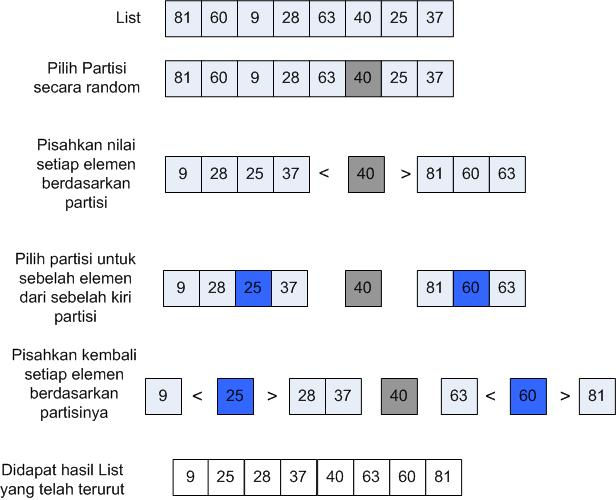
\includegraphics[scale=0.8]{fig/sunario-3/QuickSort.jpg}%
	\caption{Ilustrasi Quick Sort}%
	\label{fig:Quick Sort Ilustration}%
\end{center}
\end{figure}

Kerugian dari versi sederhana diatas adalah membutuhkan ruang simpan yang lebih besar, yang sama buruknya seperti merge sort. Memory tambahan yang dibutuhkan dapat juga secara radikal berpengaruh pada kecepatan dan performa cache pada implementasi praktiknya. Terdapat juga versi yang lebih rumit yang menggunakan algoritma partisi \textit{in-place}. Ilustrasi dari algoritma \textit{quick sort} dengan partisi \textit{in-place}. Algoritma partisi \textit{in-place} digunakan untuk memisahkan bagian dari list antara index kiri dan kanan, dengan memindahkan seluruh elemen kurang dari MyList[pivotIndex] sebelum pivot, dan elemen yang sama atau lebih besar darinya. Dalam prosesnya, algoritma ini juga mencari posisi akhir untuk elemen pivot kembali. 


Adapun ilustrasi dari cara kerja dari \textit{quick sort} dengan partisi \textit{in-place} dapat dilihat pada Figur \ref{fig:Quick Sort Ilustration 2} berikut:

\begin{figure}[htbp]
\begin{center}
	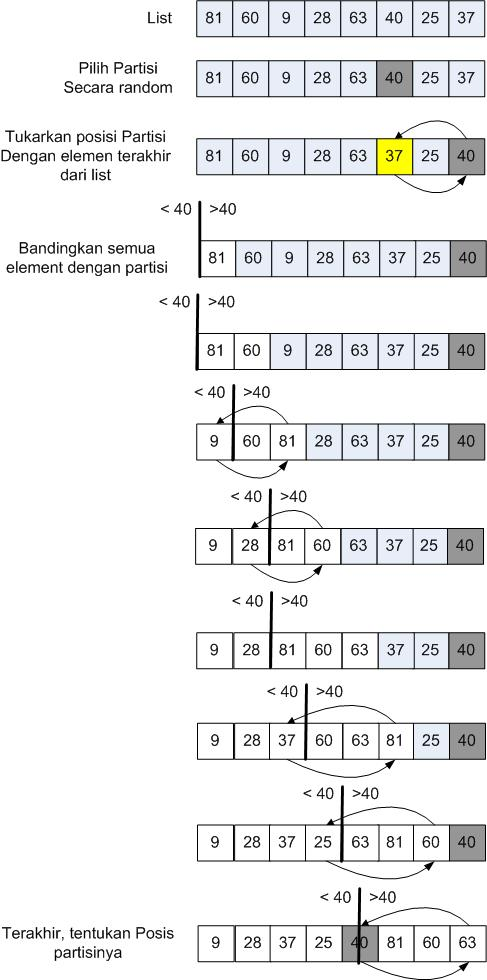
\includegraphics[scale=0.5]{fig/sunario-3/QuickSort2.jpg}%
	\caption{Ilustrasi Quick Sort In-Place}%
	\label{fig:Quick Sort Ilustration 2}%
\end{center}
\end{figure}

\newpage{}
Dalam Python Algoritma \textit{quick sort} dapat diterapkan sebagai berikut:
\lstset{language=Python}
\label{lst:QuickSort}
\begin{lstlisting}[frame=single]
def quickSort(A, p, r):
 if p < r:
   q = partition(A, p, r)
   quickSort(A, p, q-1)
   quickSort(A, q+1, r)
\end{lstlisting}

\lstset{language=Python}
\label{lst:Partition}
\begin{lstlisting}[frame=single]
def partition(A,p,r):
    x = A[r]
    i = p-1
    for j in range(p,r):
        if(A[j] <= x):
            i = i + 1
            A[i],A[j] = A[j],A[i]
    A[i+1],A[r] = A[r],A[i+1]
    return i+1
\end{lstlisting}

\subsection{Analisis Quick Sort}
Kompleksitas dari \textit{quick sort} tergantung pada  seimbang atau tidak seimbang pembagian partisi pada list yang akan diurutkan. Sebuah partisi yang  baik membagi list menjadi dua list dengan ukuran sama, sedangkan partisi yang buruk membagi list menjadi dua list dengan ukuran yang sangat berbeda. Partisi terburuk menempatkan hanya satu elemen dalam satu list dan semua elemen lainnya dalam list lain. 

Untuk menganalisi kompleksitas dari \textit{quick sort}, terlebih dahulu, perlu diperhitungkan kompleksitas dari algoritma partisi yang digunakan karena algoritma partisi yang digunakan bukan pernyataan sederhana.

\lstset{language=Python}
\label{lst:Partition}
\begin{lstlisting}[frame=single]
def partition(A,p,r):
    x = A[r]                       #cost a
    i = p-1                        #cost b
    for j in range(p,r):
        if(A[j] <= x):
            i = i + 1
            A[i],A[j] = A[j],A[i]  #cost j.n+c
    A[i+1],A[r] = A[r],A[i+1]      #cost d
    return i+1                     #cost e
\end{lstlisting}

Didalam algoritma partisi yang digunakan, terdapat sebuah loop for yang diikuti oleh statement sederhana lainnya. Statement sederhana tersebut dapat diberikan $f(n)= a+b+d+e$, kecuali yang berada di dalam statement for, dimana nilai $f(n) = j.n+c/O(n)$. Sehingga didapatkan kompleksitas untuk algoritma partisi diatas adalah :

$$ \mathnormal{f(n) = a+b+j.n+c+d+e} $$
$$ \mathnormal{f(n) = j.n} $$

Setelah mendapatkan nilai kompleksitas dari algoritma partisiya, maka dapat dihitung kompleksitas untuk algoritma \textit{quick sort} .

\lstset{language=Python}
\label{lst:QuickSort}
\begin{lstlisting}[frame=single]
def quickSort(A, p, r):
 if p < r:                #cost a
   q = partition(A, p, r) #cost j.n
   quickSort(A, p, q-1)   #cost f(n/2) + b
   quickSort(A, q+1, r)   #cost f(n/2) + c
\end{lstlisting}

yang secara matematis dapat dituliskan seperti berikut:
$$	  \mathnormal{f(n) = a+j.n+f(\frac{n}{2})+b+f(\frac{n}{2})+c } $$
$$	  \mathnormal{f(n) = 2f(\frac{n}{2})+j.n } $$

dengan syarat $n > 1$, maka:
$$	  \mathnormal{f(n) = 2f(\frac{n}{2})+j.n } $$
$$	  \mathnormal{f(n) = 2(2f(\frac{n}{4})+j.\frac{n}{2} )} + j.n $$
$$	  \mathnormal{f(n) = 4f(\frac{n}{4})+2j.n } $$
$$	  \mathnormal{f(n) = 4(2f(\frac{n}{8})+j.\frac{n}{4} )}+2j.n $$
$$	  \mathnormal{f(n) = 8f(\frac{n}{8})+3j.n } $$
$$	  \mathnormal{f(n) = 16f(\frac{n}{16})+4j.n } $$
$$	  \mathnormal{f(n) = 2^{k}f(\frac{n}{2^{k}})+k.j.n } $$

untuk $ \mathnormal{f(n) = (\frac{n}{2^{k}})} $ :

$$ \mathnormal{\frac{n}{2^{k}}=1} $$
$$ \mathnormal{2^{k}=n} $$
$$ \mathnormal{k=log_{2}n} $$

sehingga :

$$	  \mathnormal{f(n) = 2^{log_{2}n}f(1)+log_{2}n.j.n } $$

$$	  \mathnormal{f(n) = j.n\ log\ n = O(n\ log\ n)} $$

Untuk Worse Case dari \textit{quick sort} , jika partisinya dibagi tidak sama rata atau hanya satu elemen dalam satu list dan semua elemen lainnya dalam list lain seperti Figur \ref{fig:WorseCaseQuickSort}, maka kompleksitasnya adalah:

$$	  \mathnormal{f(n) = f(n-1)+j.n} $$
$$	  \mathnormal{f(n) = f(n-2)+j(n-1)+(j.n)} $$
$$	  \mathnormal{f(n) = f(n-2)+2(j.n)} $$
$$	  \mathnormal{f(n) = f(n-3)+j(n-2))+2(j.n)} $$
$$	  \mathnormal{f(n) = f(n-3)+3(j.n)} $$
$$	  \mathnormal{f(n) = f(n-4)+4(j.n)} $$
$$	  \mathnormal{f(n) = f(n-k)+k(j.n)} $$

untuk $ \mathnormal{f(n) = k.n  }$:
$$ \mathnormal{ k.n = 1  }$$
$$ \mathnormal{ k = n }$$

sehingga :

$$ \mathnormal{f(n) = f(1) + n.j.n} $$
$$ \mathnormal{f(n) = j.n^{2} = O(n^{2})} $$
		

\begin{figure}[htbp]
\begin{center}
	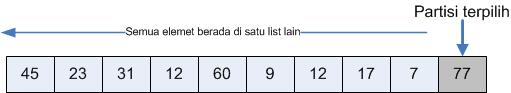
\includegraphics[scale=0.5]{fig/sunario-3/QuickSort3.jpg}%
	\caption{Quick Sort Worse Case}%
	\label{fig:WorseCaseQuickSort}%
\end{center}
\end{figure}


Jika partisi seimbang, maka kompleksitas dari  \textit{quick sort} berjalan secepat merge sort $O(n\ log\ n)$. Di sisi lain, jika partisi tidak seimbang, \textit{quick sort} berjalan lambat seperti insertion sort $O(n^{2})$.